\documentclass[12pt]{article}
\usepackage[top=1in, bottom=1in, left=.75in, right=.75in]{geometry}
\usepackage{amsmath, enumerate}
\usepackage{fancyhdr}
\usepackage{graphicx, xcolor, setspace}
\usepackage{txfonts}
\usepackage{multicol,coordsys,pgfplots}
\usepackage[scaled=0.86]{helvet}
\renewcommand{\emph}[1]{\textsf{\textbf{#1}}}
\usepackage{anyfontsize}
% \usepackage{times}
% \usepackage[lf]{MinionPro}
\usepackage{tikz,pgfplots}
\def\ra{\rightarrow}
\newcommand{\blank}[1]{\rule{#1}{0.75pt}}
\usetikzlibrary{calc,trees,positioning,arrows,fit,shapes,calc}
\pgfplotsset{width=9cm,compat=1.9}
\tikzset{
  jumpdot/.style={mark=*,solid},
  excl/.append style={jumpdot,fill=white},
  incl/.append style={jumpdot,fill=black},
}

\pgfplotsset{my style/.append style={axis x line=middle, axis y line=
middle, xlabel={$x$}, ylabel={$y$}}}

%axis equal

%yticklabels={,,} , xticklabels={,,}

% \setmainfont{Times}
% \def\sansfont{Lucida Grande Bold}
\parindent 0pt
\parskip 4pt
\pagestyle{fancy}
\fancyfoot[C]{\emph{\thepage}}
\fancyfoot[R]{v1} %%%%%% <-- Version Info
\fancyhead[L]{\ifnum \value{page} > 1\relax\emph{Math F251X: Midterm 1}\fi}
\fancyhead[R]{\ifnum \value{page} > 1\relax\emph{Spring 2025}\fi}
\headheight 15pt
\renewcommand{\headrulewidth}{0pt}
\renewcommand{\footrulewidth}{0pt}
\let\ds\displaystyle
\def\continued{{\emph {Continued....}}}
\def\continuing{{\emph {Problem \arabic{probcount} continued....}}\par\vskip 4pt}


\newcounter{probcount}
\newcounter{subprobcount}
\newcommand{\thesubproblem}{\emph{\alph{subprobcount}.}}
\def\problem#1{\setcounter{subprobcount}{0}%
\addtocounter{probcount}{1}{\emph{\arabic{probcount}.\hskip 1em(#1)}}\par}
\def\subproblem#1{\par\hangindent=1em\hangafter=0{%
\addtocounter{subprobcount}{1}\thesubproblem\emph{#1}\hskip 1em}}
\def\probskip{\vskip 10pt}
\def\medprobskip{\vskip 2in}
\def\subprobskip{\vskip 45pt}
\def\bigprobskip{\vskip 4in}


\newenvironment{subproblems}{%
\begin{enumerate}%
\setcounter{enumi}{\value{subprobcount}}%
\renewcommand{\theenumi}{\emph{\alph{enumi}}}}%
{\setcounter{subprobcount}{\value{enumi}}\end{enumerate}}


\newcommand{\be}{\begin{enumerate}}
\newcommand{\ee}{\end{enumerate}}


\begin{document}
{\emph{\fontsize{26}{28}\selectfont Spring 2026 \hfill
%{\fontsize{32}{36}\selectfont Calculus 1: Midterm 1}
\hfill Math F251X}}

\begin{center}
{\emph{%\fontsize{26}{28}\selectfont Spring 2024 
%%\hfill
{\fontsize{32}{36}\selectfont Calculus 1: Midterm 1}
%%\hfill Math F251X}
}}
\end{center}

%\vskip 2cm
\strut\vtop{\halign{\emph#\hskip 0.5em\hfil&#\hbox to 2in{\hrulefill}\cr
\emph{\fontsize{18}{22}\selectfont Name:}&\cr
%\noalign{\vskip 10pt}
%\emph{\fontsize{18}{22}\selectfont Student Id:}&\cr
%\noalign{\vskip 10pt}
%\emph{\fontsize{18}{22}\selectfont Calculator Model:}&\cr
}}
\hfill
\vtop{\halign{\emph{\fontsize{18}{22}\selectfont #}\hfil& \emph{\fontsize{18}{22}\selectfont\hskip 0.5ex $\square$ #}\hfil\cr
Section: & 9:15am (James Gossell)\cr
\noalign{\vskip 4pt}
         & 11:45am (Gordon Williams)\cr
%\noalign{\vskip 4pt}
%         & 11:45am (Margaret Short)\cr
\noalign{\vskip 4pt}
         & async (James Gossell)\cr}}
\vfill
{\fontsize{18}{22}\selectfont\emph{Rules:}}

\begin{itemize}
\item You will have $90$ minutes to take this exam.

\item Partial credit will be awarded, but you must show your work.

\item You may have a single handwritten $3'' \times 5''$ notecard, both sides.

\item Calculators are {\bf not} allowed. 

\item Place a box around your \fbox{FINAL ANSWER} to each question where appropriate.

\item Turn off anything that might go beep during the exam.

\end{itemize}

%If you need extra space, you can use the back sides of the pages.
%Please make it obvious  when you have done so.



Good luck!
\vfill
\def\emptybox{\hbox to 2em{\vrule height 16pt depth 8pt width 0pt\hfil}}
\def\tline{\noalign{\hrule}}
\centerline{\vbox{\offinterlineskip
{
\bf\sf\fontsize{18pt}{22pt}\selectfont
\hrule
\halign{
\vrule#&\strut\quad\hfil#\hfil\quad&\vrule#&\quad\hfil#\hfil\quad
&\vrule#&\quad\hfil#\hfil\quad&\vrule#\cr
height 3pt&\omit&&\omit&&\omit&\cr
&Problem&&Possible&&Score&\cr\tline
height 3pt&\omit&&\omit&&\omit&\cr
&1&&16&&\emptybox&\cr\tline
&2&&8&&\emptybox&\cr\tline
&3&&16&&\emptybox&\cr\tline
&4&&10&&\emptybox&\cr\tline
&5&&10&&\emptybox&\cr\tline
&6&&12&&\emptybox&\cr\tline
&7&&16&&\emptybox&\cr\tline
&8&&12&&\emptybox&\cr\tline
&Extra Credit&&(5)&&\emptybox&\cr\tline
&Total&&100&&\emptybox&\cr
}\hrule}}}

\newpage
\ 
\newpage
\problem{16 points} Use the graph of $f(x)$ to answer the following questions.
%Begin picture
\begin{center}
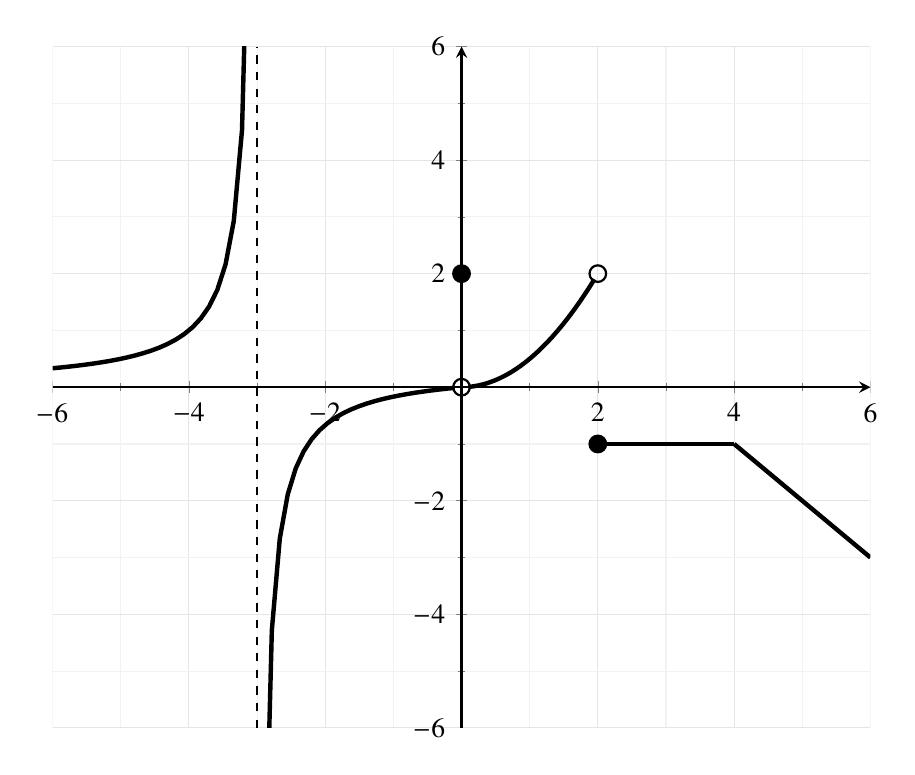
\begin{tikzpicture}
\begin{axis}[
    scale=1.4,
    axis lines=middle,
    xmin=-6, xmax=6,
    ymin=-6, ymax=6,
    xtick={-6,-4,-2,0,2,4,6},
    ytick={-6,-4,-2,0,2,4,6},
    minor x tick num=1,
    minor y tick num=1,
    grid=both,
    grid style={gray!20},
    minor grid style={gray!10},
    thick
]

% --- Jump mirrored (original at x=-2) now at x=2 ---
\addplot[ultra thick, domain=4:6, -] {-x+3};
\addplot[ultra thick, domain=2:4, -] {-1};
\addplot[ultra thick, domain=0.1:1.95] {x*x/2};

% Closed and open circles at the jump (mirror)
\addplot[only marks, mark=*, mark size=3pt] coordinates {(2,-1)};
\addplot[only marks, mark=o, mark size=3pt] coordinates {(2,2)};

% --- Hole at x = 0 (unchanged) ---
\addplot[ultra thick, domain=-2.9:-0.1] {1/(-x-3)+1/3};
\addplot[only marks, mark=o, mark size=3pt] coordinates {(0,0)};

% Floating point at (0,2) (unchanged)
\addplot[only marks, mark=*, mark size=3pt] coordinates {(0,2)};

% --- Vertical asymptote at x=-3 (mirror of original at x=3) ---
\addplot[dashed, thick] coordinates {(-3,-6) (-3,6)};
\addplot[ultra thick, domain=-6:-3.1, ->] {1/(-x-3)};

\end{axis}
\end{tikzpicture}
\end{center}
\subproblem{} Fill in the blanks below. If the value does not exist or is undefined, write DNE.\\

\begin{center} \begin{tabular}{lllll}
$\ds \lim_{x \to -3^-} f(x) =$ \blank{0.5in} && $\ds \lim_{x \to 0} f(x) =$ \blank{0.5in} && $f(0)=$ \blank{0.5in}\\
&&&&\\
$\ds \lim_{x \to 2^-} f(x) =$ \blank{0.5in}&& $\ds \lim_{x \to 2^+} f(x) =$\blank{0.5in}&& $\ds \lim_{x \to 2} f(x) =$ \blank{0.5in}\\
&&&&\\
$\ds f'(3)=$ \blank{0.5in}&& $\ds \lim_{x \to 4^-} f'(x) =$\blank{0.5in}&& $\ds \lim_{x \to -4^+} f'(x) =$ \blank{0.5in}\\
\end{tabular} \end{center}
\vfill
\subproblem{} State the $x$-values for which $f$ is \emph{not continuous}. For each of your answers, classify the discontinuity as \emph{jump}, \emph{removable}, \emph{infinite}, or \emph{other}.\\
 

\vfill
	\subproblem{} State the $x$-values for which $f$ is \emph{not differentiable} (where $f'(x)$ does not exist).\\
	\vfill
\newpage

\problem{8 points} %2.1
The distance $d$ in centimeters of a ball from a wall at time $t$ is given by $\displaystyle d(t)=10+3\cos\left(\frac{5\pi}{3}t\right)$, where $t$ is measured in seconds. We are interested in the velocity of the ball after one second.\\


In the table below, $v_{\text{avg}}$ denotes the average velocity of the ball on the time interval between the time 1 second, and the time $t$ seconds. Note that $d(1)=23/2$.


%\begin{table}[htp]
%\caption{default}
%\begin{center}
%\begin{tabular}{|c|c|}
%
%\end{tabular}
%\end{center}
%\label{default}
%\end{table}%

\begin{tabular}{l|l|l}
$t$ sec & $d(t)$ cm & $v_{\text{avg}}$ cm/sec\\
\hline\hline
0.00000 & &  \\
&& \\\hline
0.9 & 10. & 15. \\\hline
0.99 & 11.362 & 13.8029 \\\hline
0.999 & 11.4864 & 13.624 \\\hline
0.9999 & 11.4986 & 13.6056 \\\hline
0.99999 & 11.4999 & 13.6037 \\\hline
1.00001 & 11.5001 & 13.6033 \\\hline
1.0001 & 11.5014 & 13.6014 \\\hline
1.001 & 11.5136 & 13.5829 \\\hline
1.01 & 11.6339 & 13.3917 \\\hline
1.1 & 12.5981 & 10.9808 \\\hline
2 & 17/2 & -3 \\
\end{tabular}

\begin{subproblems}
\item Fill in the missing entries in the table above (for $t=0.00000$ seconds).

\vspace{0.5in}
\item Using the data provided in the table above, estimate a value for the instantaneous velocity of the ball when $t=1$ second.

\vfill
\item Is the ball moving towards the wall, or away from the wall when $t=1$ second?
\vfill

\end{subproblems}
\newpage
\problem{16 points} 
Evaluate the following limits. Show your work. Use limit notation where necessary; you will be graded
both on your computation and on your correct use of notation.
If the limit does not exist, write DNE and a few words about why it does not exist. If the limit is unbounded, write $\infty$ or $-\infty$ as appropriate, and again, justify your answer with a few words.
\begin{subproblems}
\item $\displaystyle\lim_{x\to -3} \frac{\sqrt{x+4}-1}{x+3}$
\vfill
\vfill
\vfill
\item $\displaystyle\lim_{t\to 2}\dfrac{\frac{1}{2}-\frac{1}{t}}{t-2}$
\vfill
\vfill
\vfill
\item $\displaystyle\lim_{\theta\to 0}\frac{2\theta}{\cos(\theta)}$
\vfill
\vfill
\item $\displaystyle\lim_{x\to 1^{+}}\frac{2xe^{-x}}{x^{2}(1-x)}$
\vfill
\vfill
\end{subproblems}

\newpage

\problem{10 points} Consider the function \[f(x)=x^{2}+3x.\]
Find $f'(-2)$ using the \emph{limit definition of the derivative} and show your work using all appropriate notation. \emph{No credit will be awarded for using other methods}. Begin by writing down the limit definition of the derivative. You must write limits where necessary to receive full credit.
\newpage

\problem{10 points} The graph of $f(x)$ is shown below. On the \emph{other set of axes}, sketch the graph of $f'(x)$. If there are any asymptotes, draw them with dashed lines. Use open circles to show points where the derivative is not defined, if any. (You are not given values on the $y$-axis; I am interested in the correct shape/holes/asymptotes of the derivative, not the specific values.)
\begin{center}
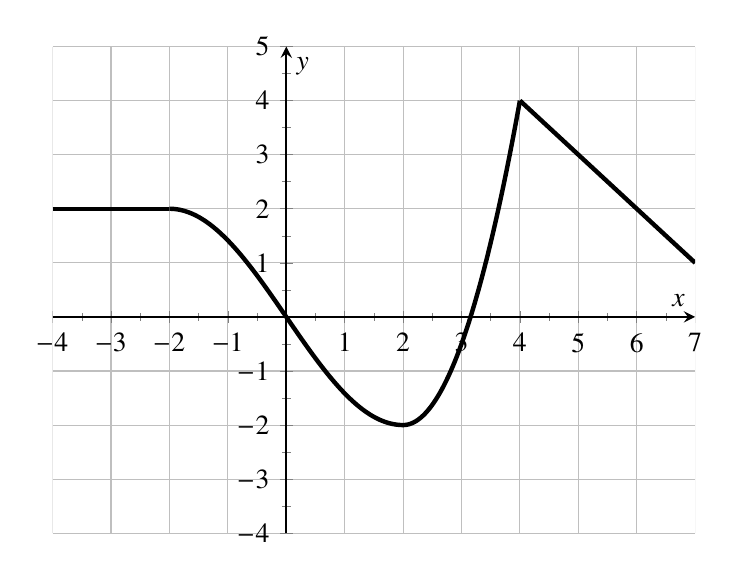
\begin{tikzpicture}
%cubic
\begin{axis}[xscale=1.1, thick, my style, xtick={-4,-3,-2,...,3,4,5, 6, 7}, ytick={-4,-3,...,5},xmin=-4, xmax=7, ymin=-4, ymax=5, minor y tick num=1, minor x tick num=1, 
mark size=3.0pt, grid = major]
\addplot[ultra thick, -,domain=-4:-1, samples=100]coordinates{(-4,2)(-2,2)};
\addplot[ultra thick, samples=200, domain=-2:2] {-2*sin(deg(pi*x/4))};
\addplot[ultra thick, samples=200, domain=2:4] {3/2*(x-2)^2 - 2};
\addplot[ultra thick, -,domain=-4:-1, samples=100]coordinates{(4,4)(7,1)};
\end{axis}
\end{tikzpicture}%
\hfill
\begin{tikzpicture}
\begin{axis}[xscale=1.1, thick, my style, xtick={-4,-3,-2,...,3,4,5, 6, 7}, ytick={0},
xmin=-4, xmax=7, ymin=-4, ymax=5, minor y tick num=0, minor x tick num=1, 
mark size=3.0pt, grid = none]
\end{axis}
\end{tikzpicture}
\end{center}

\problem{12 points} Find the derivatives of the following functions. Use appropriate derivative notation (like ``$f'(x)=$'').

\begin{subproblems}
	\item $f(x)=x^4+4x+\dfrac{1}{x^4}+\cos\left(\frac{\pi}{4}\right)$
	
	\vfill
	
	\item $g(x)=\dfrac{x^2\sin(x)}{2x-1}$
	
	\vfill
	
	\item $h(x)=\sqrt{x}(x^2-7x+12)$
	
	\vfill
\end{subproblems}

\newpage

\problem{16 points} A drone is launched from the ground. Its \emph{height} (in feet) at time $t$ seconds is given by the function $h(t)=\dfrac{32t}{t+1}$.

\begin{subproblems}
	\item What is the \emph{initial velocity} of the drone?
	
	\vfill
	
	\item After $3$ seconds, what is the \emph{velocity} of the drone?
	
	\vfill
	
	\item Someone has determined that the acceleration of the drone  at time $t$ seconds is given by \[a(t)=-\dfrac{64}{(t+1)^{3}}.\]Describe in a sentence how they obtained the acceleration from $h(t)$.
	%After $3$ seconds, what is the \emph{acceleration} of the drone?
	
	\vfill

	\item Is the drone speeding up or slowing down when $t=3$ seconds? Explain your reasoning.

	\vfill
\end{subproblems}

\newpage

\problem{12 points} A machine extrudes a metal onto a conveyor belt. Let $M(l)$ denote the amount of mass measured in kilograms extruded after the machine has travelled $l$ meters along the belt.
\begin{subproblems}
\item What does $\displaystyle \frac{M(b)-M(a)}{b-a}$ for $0<a<b$ measure, and what are the units?
\vfill
\item What does $M'(l)$ measure, and what are the units?
\vfill
\item Suppose that $M(4)=152$, and $M'(4)=13$. Estimate $M(5)$. Be sure to include appropriate units in your answer.
\vfill
\item Can $M'(l)$ be negative? Explain your reasoning.
\vfill
\end{subproblems}
\newpage
\problem{Extra Credit: 5 points} 
Suppose that \[g(x)=\begin{cases} 
4x-x^{2} & x\le 3\\
9-2x & x>3
\end{cases}.\]
Is the $g(x)$ differentiable at $x=3$? (In other words, does $g'(3)$ exist?) If so, what is $g'(3)$? 

Either way, justify your conclusions.
\end{document}

%%%%ENDDOCUMENT


